% Homework template for Automaton and Formal Logic
% UPDATE: September 20, 2019 by Xu Rongchen
\documentclass[a4paper]{article}
\usepackage{ctex}
\ctexset{
proofname = \heiti{证明} %% set proof name
}
\usepackage{amsmath, amssymb, amsthm}
% amsmath: equation*, amssymb: mathbb, amsthm: proof
\usepackage{moreenum}
\usepackage{mathtools}
\usepackage{url}
\usepackage{bm}
\usepackage{enumitem}
\usepackage{graphicx}
\usepackage{subcaption}
\usepackage{booktabs} % toprule
\usepackage[mathcal]{eucal}
\usepackage{longtable}
\usepackage[thehwcnt = 2]{iidef} % set homework count

\usepackage{tikz}
\usetikzlibrary{automata}

\thecoursename{自动机与形式逻辑}
\theterm{2019年秋季学期}
% \hwname{作业}
\slname{\heiti{解}}
\begin{document}
\courseheader
\theusername{徐荣琛}
\thestuno{2019214528}
\theinstitute{软件学院}

\info

\begin{enumerate}
  \setlength{\itemsep}{3\parskip}
  %% Homework Start here:
  %% \item to enumerate the problem ID: Format as 'HomeworkID.ProblemID'
  %% \begin{solution} XXXX \end{solution} is to make a solution
  %% \begin{proof} XXXX \end{proof} is to make a proof
  %% Suggest to use \input{path} command
  \item \textbf{[Exercise 5.1.1]} Design context-free grammar for the following languages:\\
b) The set $\{a^ib^jc^k \mid i \neq j or j \neq k\}$, that is, the set of strings
of $a$'s followed by $b$'s followed $c$'s, such that there are either a different
number of $a$'s and $b$'s or a different number of $b$'s and $c$'s, or both.
  \begin{solution}
    (1)约定谓词$P(x)$:$x$是乌鸦,$Q(x,y)$:$x$、$y$的黑度相同。
    $$\forall x,y (P(x)\wedge P(y)\rightarrow Q(x,y))$$
    (2)约定谓词$P(x)$:$x$是筵席,$Q(x)$:$x$能够结束。
    $$\forall x (P(x)\rightarrow Q(x))$$
    (3)约定谓词$P(x)$:$x$是金子,$Q(x)$:$x$能够闪光。
    $$\exists x (\neg P(x) \wedge Q(x))$$
    (4)约定谓词$P(x)$:$x$是奇数,$Q(x)$:$x$是素数。
    $$\exists x (\neg P(x) \wedge Q(x))$$
    (5)约定谓词$P(x)$:$x$是偶数,$Q(x)$:$x$是素数,$R(x,y)$:$x$、$y$相等。
    $$\forall x,y (P(x)\wedge Q(x)\wedge P(y)\wedge Q(y)\rightarrow R(x,y))$$
    (6)约定谓词$P(x)$:$x$是猫,$Q(x)$:$x$是动物。
    $$(\forall x (P(x)\rightarrow Q(x)))\wedge \neg(\forall x (Q(x)\rightarrow P(x)))$$
    (7)约定谓词$P(x)$:$x$ is mushroom,$Q(x)$:$x$ is purple,$R(x)$:$x$ is poisonous。
    $$\neg \exists (x P(x)\wedge Q(x)\wedge R(x))$$
    (8)约定谓词$P(x)$:$x$ is mushroom,$Q(x)$:$x$ is purple,$R(x,y)$:$x$, $y$ is same。
    \begin{align*}
        &\exists x,y(P(x)\wedge Q(x)\wedge P(y)\wedge Q(y)\wedge \neg R(x,y) \wedge \\
        &\forall z(P(z)\wedge Q(z)\rightarrow (R(x,z)\vee R(y,z))))
    \end{align*}
\end{solution}
  \item 设字母表为$\{0,1\}$. 给出接受所有倒数第3个符号是1的语言的DFA.
  \begin{solution}DFA转移表:
\begin{center}
    \begin{tabular}{r||l|l||r||l|l}
                        & $0$           & $1$   & ~             & $0$           & $1$\\ \hline \hline
        $\rightarrow p$ & $qs$          & $q$   & $*qs$         & $r$           & $pqr$\\
        $*q$            & $r$           & $qr$  & $*rs$         & $s$           & $p$\\
        $r$             & $s$           & $p$   & $*pqr$        & $qrs$         & $pqr$\\
        $*s$            & $\emptyset$   & $p$   & $*qrs$        & $rs$          & $pqr$\\
        $*qr$           & $rs$          & $pqr$ & $\emptyset$   & $\emptyset$   & $\emptyset$\\
        
    \end{tabular}
\end{center}
    % 如图所示:\\
    % \begin{tikzpicture}
        
    %     % \draw[help lines] (0,0) grid (10,-5);
    %     \node[state,initial,initial text={}] at (1,0) (p){$\{p\}$};
    %     \node[state,accepting,minimum size=40] at (5,0) (q){$\{q\}$};
    %     \node[state] at (7,0) (r){$\{r\}$};
    %     \node[state,accepting] at (1,-2) (qs){$\{q,s\}$};
    %     \node[state,accepting] at (1,-4) (qr){$\{q,r\}$};
    %     \node[state,accepting] at (1,-6) (pqr){$\{p,q,r\}$};
    %     \node[state,accepting] at (3,-4) (rs){$\{r,s\}$};
    %     \node[state,accepting] at (5,-4) (s){$\{s\}$};
    %     \node[state] at (7,-4) (e){$\emptyset$};

    %     \node[state,accepting] at (3,-2) (qrs){$\{q,r,s\}$};
    %     \node[state,accepting] at (5,-2) (pq){$\{p,q\}$};


    %     \path[->]
    %     (p) edge node {0} (qs)
    %     (p) edge node {1} (q)

    %     (qs) edge node {0} (r)
    %     (qs) edge node {1} (pqr)

    %     (q) edge node {0} (r)
    %     (q) edge node {1} (qr)

    %     (r) edge node {0} (s)
    %     (r) edge node {1} (p)

    %     (pqr) edge node {0} (qrs)
    %     (pqr) edge node {1} (pqr)

    %     ;
    % \end{tikzpicture}
\end{solution}
  \item Explain why the following are not well-formed CTL formulas:

(c) $\textrm{A}\neg \textrm{G}\neg p $

(e) $\textrm{EXX }r$

  \begin{proof}
    根据命题逻辑的有效性和完备性,证明$p\vdash q$ iff $\vdash(p\rightarrow q)$即可
    证明$p\models q$ iff $\models (p\rightarrow q)$。

    % 基于K,S,DN,MP公理系统进行证明:
    通过希尔伯特公理系统进行证明:
    \begin{align*}
        \text{K公理:}\; &A \rightarrow (B \rightarrow A)\\
        \text{S公理:}\; &(A \rightarrow (B \rightarrow C))\rightarrow ((A\rightarrow B)\rightarrow(A\rightarrow C))\\
        % \text{DN:}\;&\neg \neg A \rightarrow A\\
        \text{MP规则:}\; &\{A\rightarrow B,A\} \vdash  B.
    \end{align*}
    定理$\vdash  A\rightarrow A$的证明:
    \begin{align*}
        \vdash &\; (A\rightarrow ((D\rightarrow A)\rightarrow A))\rightarrow \\
            &((A\rightarrow (D\rightarrow A))\rightarrow (A\rightarrow A))
            &\text{S}(B\Leftarrow D\rightarrow A,C\Leftarrow A)\; \text{1}\\
        \vdash &\; A\rightarrow ((D\rightarrow A)\rightarrow A)&\text{K}(B\Leftarrow D\rightarrow A)\; \text{2}\\
        \vdash &\; (A\rightarrow (D\rightarrow A))\rightarrow (A\rightarrow A) &\text{MP,(1),(2)}\; \text{3}\\
        \vdash &\; A\rightarrow (D\rightarrow A) &\text{K}\;\text{4}\\
        \vdash &\; A\rightarrow A&\text{MP,(3),(4)}\; \text{5}\\
    \end{align*}
    $\vdash  (p\rightarrow q) \Rightarrow p\vdash  q$的证明:
    \begin{align*}
        \vdash &\; p\rightarrow q  &\text{[前提]\;1}\\
        % \vdash &\; \neg \neg p\rightarrow p  &\text{[DD引入]\;2}\\
        % \vdash &\; p\rightarrow p  &\text{[定理$A\rightarrow A$]\;2}\\
        % p\vdash &\; p &\text{[MP\{2, $p$\}]\;3}\\
        p\vdash &\; q &\text{[MP\{1, $p$\}] 2}\\
    \end{align*}

    $p\vdash  q \Rightarrow\; \vdash  (p\rightarrow q) $的证明:

    假设$A\vdash  B$基于演绎证明系统的一个证明序列为$B_1,B_2,\ldots,B_n$($B_n=B$)。
    
    下面采用归纳法证明$A\vdash  B \Rightarrow \; \vdash  (A\rightarrow B)$:

    \textbf{初始:} $n=1$。此时$B_1$只能有两个来源:

    \textit{初始情形1:}$B_1$是公理(包括公理的某种代入)。此时显然$\vdash  B_1$,又根据K公理可知,$\vdash  B_1\rightarrow (A \rightarrow B_1)$,
    应用MP规则,$\vdash  (A \rightarrow B_1)$;

    \textit{初始情形2:}$B_1$即$A$。此时由于定理$\vdash  A\rightarrow A$,可知$\vdash  (A \rightarrow B_1)$;
    
    于是初始$\vdash  (A \rightarrow B_1)$。

    \textbf{归纳:} $n=i$。此时$B_i$有两个来源:

    \textit{归纳情形1:}$B_i$是公理(包括公理的某种代入)或者$A$,于是同初始情形,可证$\vdash  (A \rightarrow B_i)$;

    \textit{归纳情形2:}$B_i$是$B_j,B_m$应用MP规则的归结($j<i,m<i$),假设MP$\frac{B_j;B_m}{B_i}$,另外我们已知
    $\vdash  (A \rightarrow B_j)$,以及$\vdash  (A \rightarrow B_m)$。又根据MP规则,
    不是一般性地,我们可以假定$B_m$是$B_j\rightarrow B_i$的形式,于是代入公式可得
    $\vdash  (A \rightarrow (B_j\rightarrow B_i))$。注意到,S公理的一个有效的代入是
    $\vdash  (A \rightarrow (B_j \rightarrow B_i))\rightarrow ((A\rightarrow B_j)\rightarrow(A\rightarrow B_i))$,
    于是应用MP规则,得到$\vdash  ((A\rightarrow B_j)\rightarrow(A\rightarrow B_i))$,继续利用$\vdash  (A \rightarrow B_j)$
    应用MP规则,得到$\vdash  (A \rightarrow B_i)$。

    于是归纳$\vdash  (A \rightarrow B_i)$。

    综上所述,根据初始条件和归纳条件,对于任意长度的证明序列,$A\vdash  B \Rightarrow\; \vdash  (A \rightarrow B)$。

    双向得证。
\end{proof}
  \item \textbf{[Exercise 5.2.1]} For the grammar and each of the strings in 
Exercise 5.1.2, give the parse trees.

  \begin{solution}
    c)如图所示:\\
    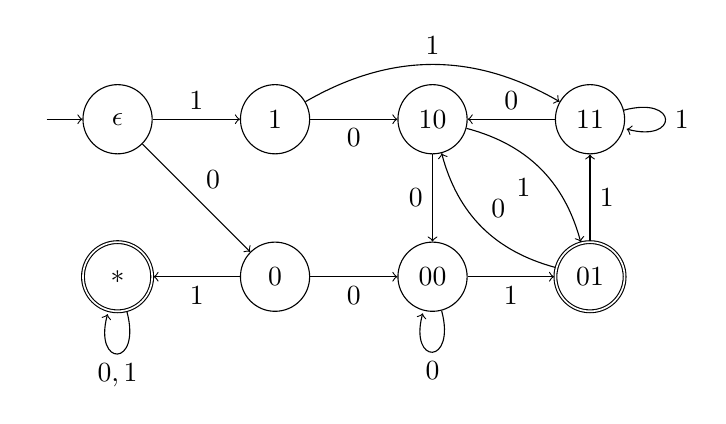
\begin{tikzpicture}
        % \draw[help lines] (0,0) grid (10,-5);
        \node[state] at (7,0) (11){$11$};
        \node[state] at (5,0) (10){$10$};
        \node[state,accepting] at (7,-2) (01){$01$};
        \node[state] at (5,-2) (00){$00$};
        
        \node[state] at (3,0) (1) {$1$};
        \node[state,initial,initial text={}] at (1,0) (e) {$\epsilon$};
        \node[state,accepting] at (1,-2) (x) {$*$};
        \node[state] at (3,-2) (0) {$0$};
        

        \path[->]
        (e) edge node [above right] {$0$} (0)
        (e) edge node [above] {$1$} (1)

        (0) edge node [below] {$0$} (00)
        (0) edge node [below] {$1$} (x)

        (1) edge node [below] {$0$} (10)
        (1) edge [bend left] node [above] {$1$} (11)

        (x) edge [loop below] node {$0,1$} (x)

        (00) edge [loop below] node {$0$} (00)
        (00) edge node [below] {$1$} (01)

        (01) edge [bend left] node [above right] {$0$} (10)
        (01) edge node [right] {$1$} (11)

        (10) edge node [left] {$0$} (00)
        (10) edge [bend left] node [below left] {$1$} (01)

        (11) edge node [above] {$0$} (10)
        (11) edge [loop right] node {$1$} (11);
    \end{tikzpicture}\\
    d)如图所示:\\
    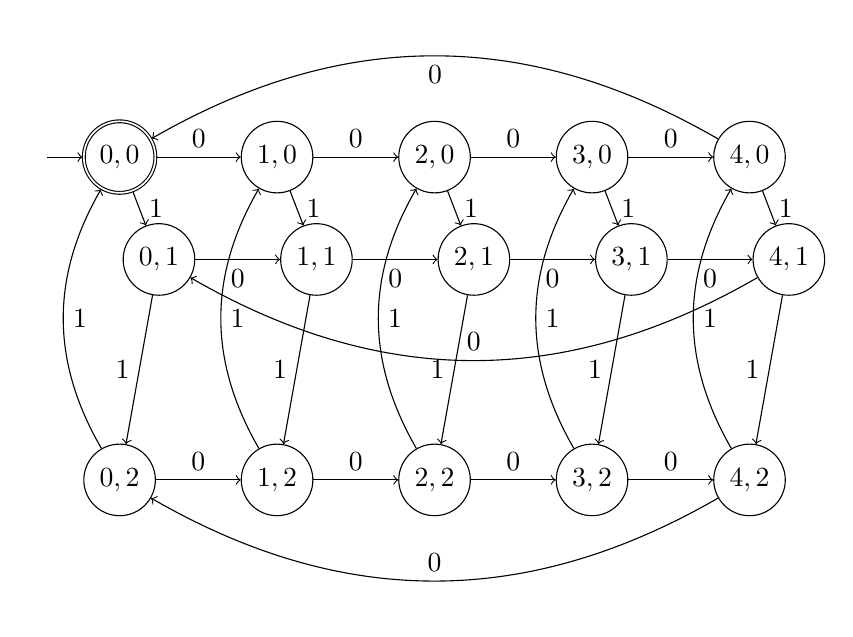
\begin{tikzpicture}
        % \draw[help lines] (0,0) grid (10,-5);
        \node[state,initial,initial text={},accepting] at (0,0) (00) {$0,0$};
        \node[state] at (2,0) (10) {$1,0$};
        \node[state] at (4,0) (20) {$2,0$};
        \node[state] at (6,0) (30) {$3,0$};
        \node[state] at (8,0) (40) {$4,0$};

        \node[state] at (0.5,-1.3) (01) {$0,1$};
        \node[state] at (2.5,-1.3) (11) {$1,1$};
        \node[state] at (4.5,-1.3) (21) {$2,1$};
        \node[state] at (6.5,-1.3) (31) {$3,1$};
        \node[state] at (8.5,-1.3) (41) {$4,1$};

        \node[state] at (0,-4.1) (02) {$0,2$};
        \node[state] at (2,-4.1) (12) {$1,2$};
        \node[state] at (4,-4.1) (22) {$2,2$};
        \node[state] at (6,-4.1) (32) {$3,2$};
        \node[state] at (8,-4.1) (42) {$4,2$};

        \path[->]
        (00) edge node [above] {$0$} (10)
        (00) edge node [right] {$1$} (01)

        (10) edge node [above] {$0$} (20)
        (10) edge node [right] {$1$} (11)

        (20) edge node [above] {$0$} (30)
        (20) edge node [right] {$1$} (21)
        
        (30) edge node [above] {$0$} (40)
        (30) edge node [right] {$1$} (31)

        (40) edge [bend right] node [below] {$0$} (00)
        (40) edge node [right] {$1$} (41)
        

        (01) edge node [below] {$0$} (11)
        (01) edge node [left] {$1$} (02)

        (11) edge node [below] {$0$} (21)
        (11) edge node [left] {$1$} (12)

        (21) edge node [below] {$0$} (31)
        (21) edge node [left] {$1$} (22)
        
        (31) edge node [below] {$0$} (41)
        (31) edge node [left] {$1$} (32)

        (41) edge [bend left] node [above] {$0$} (01)
        (41) edge node [left] {$1$} (42)
        

        (02) edge node [above] {$0$} (12)
        (02) edge [bend left] node [right] {$1$} (00)

        (12) edge node [above] {$0$} (22)
        (12) edge [bend left] node [right] {$1$} (10)

        (22) edge node [above] {$0$} (32)
        (22) edge [bend left] node [right] {$1$} (20)
        
        (32) edge node [above] {$0$} (42)
        (32) edge [bend left] node [right] {$1$} (30)

        (42) edge [bend left] node [above] {$0$} (02)
        (42) edge [bend left] node [right] {$1$} (40);

    \end{tikzpicture}
\end{solution}
  \item \textbf{思考题[Exercise 2.2.5]} Give DFA's accepting the following languages 
over the alphabet $\{0,1\}$:\\
a) The set of all strings such that each block of five consecutive 
symbols contains at least two $0$'s.\\
b) The set of strings whose tenth symbol from the right end is a $1$.

  \begin{solution}
    最左推导:
    \begin{align*}
        E &\Rightarrow +EE \Rightarrow +* EEE \Rightarrow +*- EEEE \Rightarrow +*- xEEE\\
        &\Rightarrow +*- xyEE  \Rightarrow +*- xyxE \Rightarrow +*- xyxy
    \end{align*}
    最右推导:
    \begin{align*}
        E &\Rightarrow +EE \Rightarrow + Ey \Rightarrow +* EEy \Rightarrow +* Exy\\
        &\Rightarrow +*- EExy  \Rightarrow +*- Eyxy \Rightarrow +*- xyxy
    \end{align*}
    推导树:
    \begin{center}
        \begin{tikzpicture} 
            \node {$E$} 
                child { node {$+$} }
                child { 
                    node {$E$} 
                    child { node {$*$} }
                    child { 
                        node {$E$}
                        child { node {$-$} }
                        child { 
                            node {$E$} 
                            child { node {$x$} }
                        }
                        child { 
                            node {$E$} 
                            child { node {$y$} }
                        } 
                    }
                    child { 
                        node {$E$} 
                        child { node[right=35] {$x$} }
                    }
                }
                child { 
                    node {$E$} 
                    child { node[right=35] {$y$} }
                }
                ; 
        \end{tikzpicture}
    \end{center}
\end{solution}
  \item \textbf{[Exercise 7.1.9]} Provide the inductive proofs needed to complete
the following theorems:

b) Both directions of Theorems 7.6, where we show the correctness
of the algorithm in Section 7.1.2 for detecting the reachable symbols.
  \begin{solution}
    a) $p$,$q$,$r$的$\epsilon$闭包:\\
    $ECLOSE(p) = \{p\}$\\
    $ECLOSE(q) = \{p,q\}$\\
    $ECLOSE(r) = \{p,q,r\}$\\
    b) 自动机所接受的长度3以下的串有:\\
    c, ac, bb, bc, cb, cc,\\
    aac, abb, abc, aca, acb, acc,\\
    bab, bac, bba, bbb, bbc, bca, bcb, bcc,\\
    caa, cab, cac, cba, cbb, cbc, cca, ccb, ccc

    a)如图所示\\
    \bigskip
    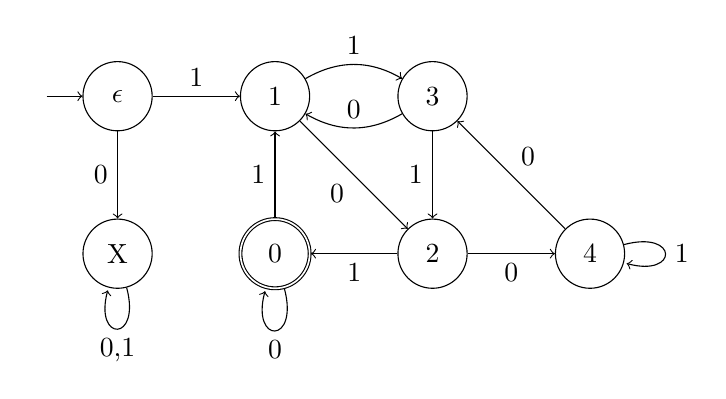
\begin{tikzpicture}
        \node[state,initial, initial text={}] at (0,0) (e) {$\epsilon$};

        \node[state] at (0,-2) (x) {X};

        \node[state,accepting] at (2,-2) (0) {0};
        \node[state] at (2,0) (1) {1};
        \node[state] at (4,-2) (2) {2};
        \node[state] at (4,0) (3) {3};
        \node[state] at (6,-2) (4) {4};

        \path[->]
        (e) edge node [left] {0} (x)
        (e) edge node [above] {1} (1)
        
        (x) edge [loop below] node {0,1} (x)

        (0) edge [loop below] node {0} (0)
        (0) edge node [left] {1} (1)

        (1) edge node [below left] {0} (2)
        (1) edge [bend left] node [above] {1} (3)

        (2) edge node [below] {0} (4)
        (2) edge node [below] {1} (0)

        (3) edge [bend left] node [above] {0} (1)
        (3) edge node [left] {1} (2)

        (4) edge node [above right] {0} (3)
        (4) edge [loop right] node {1} (4)
        ;
    \end{tikzpicture}
    \clearpage
    b)如图所示:\\
    \bigskip
    \resizebox{320pt}{320pt}{%
    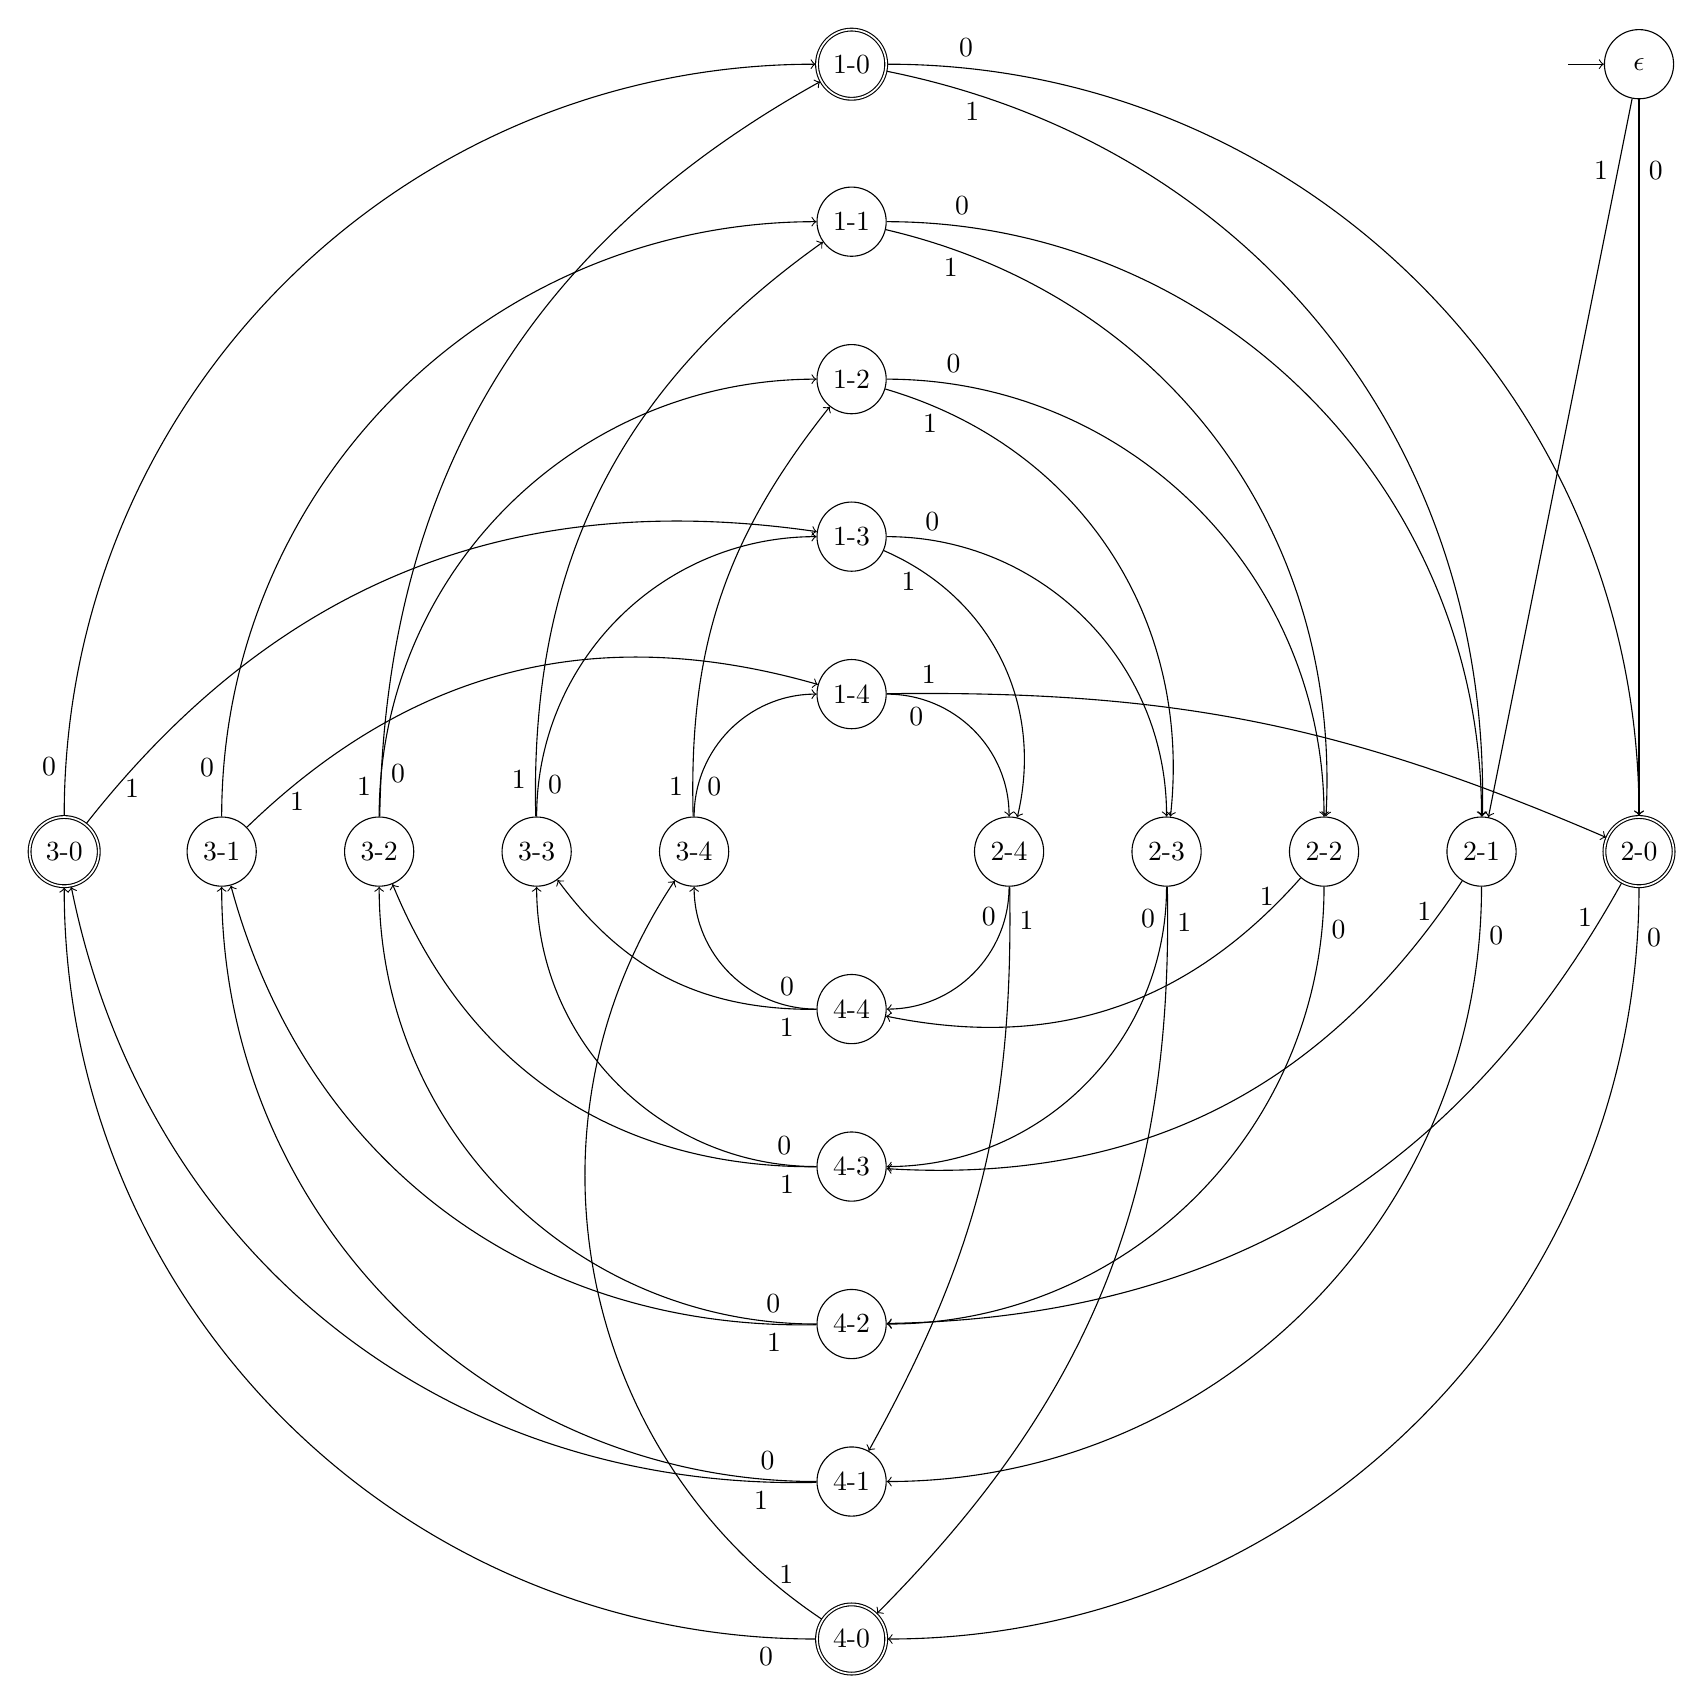
\begin{tikzpicture}
        \node[state,initial,initial text={}] at(10,10) (e) {$\epsilon$};
        
        \node[state] at (-2,0) (3-4) {3-4};
        \node[state] at (-4,0) (3-3) {3-3};
        \node[state] at (-6,0) (3-2) {3-2};
        \node[state] at (-8,0) (3-1) {3-1};
        \node[state,accepting] at (-10,0) (3-0) {3-0};

        \node[state] at (0,-2) (4-4) {4-4};
        \node[state] at (0,-4) (4-3) {4-3};
        \node[state] at (0,-6) (4-2) {4-2};
        \node[state] at (0,-8) (4-1) {4-1};
        \node[state,accepting] at (0,-10) (4-0) {4-0};

        \node[state] at (2,0) (2-4) {2-4};
        \node[state] at (4,0) (2-3) {2-3};
        \node[state] at (6,0) (2-2) {2-2};
        \node[state] at (8,0) (2-1) {2-1};
        \node[state,accepting] at (10,0) (2-0) {2-0};

        \node[state] at (0,2) (1-4) {1-4};
        \node[state] at (0,4) (1-3) {1-3};
        \node[state] at (0,6) (1-2) {1-2};
        \node[state] at (0,8) (1-1) {1-1};
        \node[state,accepting] at (0,10) (1-0) {1-0};

        \path[->]
        (e) edge node [right,pos=0.1] {0} (2-0)
        (e) edge node [left,pos=0.1] {1} (2-1)

        (1-0) edge [bend left=45] node [above right,pos=0.05] {0} (2-0)
        (1-1) edge [bend left=45] node [above right,pos=0.06] {0} (2-1)
        (1-2) edge [bend left=45] node [above right,pos=0.07] {0} (2-2)
        (1-3) edge [bend left=45] node [above,pos=0.1] {0} (2-3)
        (1-4) edge [bend left=45] node [below,pos=0.15] {0} (2-4)
        
        (2-0) edge [bend left=45] node [right,pos=0.04] {0} (4-0)
        (2-1) edge [bend left=45] node [right,pos=0.05] {0} (4-1)
        (2-2) edge [bend left=45] node [right,pos=0.06] {0} (4-2)
        (2-3) edge [bend left=45] node [left,pos=0.07] {0} (4-3)
        (2-4) edge [bend left=45] node [left,pos=0.15] {0} (4-4)

        (4-0) edge [bend left=45] node [below,pos=0.04] {0} (3-0)
        (4-1) edge [bend left=45] node [above,pos=0.05] {0} (3-1)
        (4-2) edge [bend left=45] node [above,pos=0.06] {0} (3-2)
        (4-3) edge [bend left=45] node [above,pos=0.07] {0} (3-3)
        (4-4) edge [bend left=45] node [above,pos=0.15] {0} (3-4)

        (3-0) edge [bend left=45] node [left,pos=0.04] {0} (1-0)
        (3-1) edge [bend left=45] node [left,pos=0.05] {0} (1-1)
        (3-2) edge [bend left=45] node [right,pos=0.06] {0} (1-2)
        (3-3) edge [bend left=45] node [right,pos=0.07] {0} (1-3)
        (3-4) edge [bend left=45] node [right,pos=0.15] {0} (1-4)

        (1-0) edge [bend left=40] node [below,pos=0.08] {1} (2-1)
        (1-1) edge [bend left=40] node [below,pos=0.08] {1} (2-2)
        (1-2) edge [bend left=40] node [below,pos=0.08] {1} (2-3)
        (1-3) edge [bend left=40] node [below,pos=0.08] {1} (2-4)
        (1-4) edge [bend left=12] node [above,pos=0.05] {1} (2-0)
        
        (2-0) edge [bend left=30] node [left,pos=0.04] {1} (4-2)
        (2-1) edge [bend left=30] node [left,pos=0.05] {1} (4-3)
        (2-2) edge [bend left=30] node [left,pos=0.05] {1} (4-4)
        (2-3) edge [bend left=23] node [right, pos=0.04] {1} (4-0)
        (2-4) edge [bend left=15] node [right, pos=0.05] {1} (4-1)

        (4-0) edge [bend left=45] node [above,pos=0.05] {1} (3-4)
        (4-1) edge [bend left=40] node [below,pos=0.05] {1} (3-0)
        (4-2) edge [bend left=38] node [below,pos=0.05] {1} (3-1)
        (4-3) edge [bend left=34] node [below,pos=0.05] {1} (3-2)
        (4-4) edge [bend left=27] node [below,pos=0.09] {1} (3-3)

        (3-0) edge [bend left=30] node [right,pos=0.05] {1} (1-3)
        (3-1) edge [bend left=30] node [below,pos=0.1] {1} (1-4)
        (3-2) edge [bend left=30] node [left,pos=0.03] {1} (1-0)
        (3-3) edge [bend left=28] node [left,pos=0.05] {1} (1-1)
        (3-4) edge [bend left=20] node [left,pos=0.06] {1} (1-2)

        ;
    \end{tikzpicture}
    }
\end{solution}

\end{enumerate}

\end{document}


%%% Local Variables:
%%% mode: late\rvx
%%% TeX-master: t
%%% End:
